\documentclass[a4paper,onecolumn]{report}
\usepackage{caption}
\usepackage{subcaption}
\usepackage{setspace}
\usepackage{amssymb}
\usepackage[fleqn]{amsmath}
\usepackage{cite}
\usepackage{graphicx}
\usepackage{color}
\usepackage{float}
\usepackage[toc,page]{appendix}
\usepackage[nottoc]{tocbibind}
\usepackage{titlesec}
\usepackage{float}
\usepackage{setspace}
\usepackage{comment}
\titleformat{\chapter}{\normalfont\huge}{\thechapter.}{15pt}{\huge}
\renewcommand*{\familydefault}{\sfdefault}
\hyphenpenalty=5000 
\tolerance=1000

\usepackage[a4paper]{geometry}
\voffset=-80pt
\hoffset=0pt
\topmargin = 0pt
\textwidth = 450pt
\textheight = 770pt
\marginparwidth = 10pt
\oddsidemargin = 5pt
\topmargin = 1pt
\graphicspath{ {/images/} }

\setcounter{tocdepth}{2}

\begin{document}

%----------------------------------------------------------------------------------------
%	TITLE SECTION
%----------------------------------------------------------------------------------------

\begin{titlepage}

\newcommand{\HRule}{\rule{\linewidth}{0.5mm}}
\newcommand{\horrule}[1]{\rule{\linewidth}{#1}}

\center % Center everything on the page

\textsc{\small DELFT UNIVERSITY of TECHNOLOGY}\\[2.5cm] % Name of your university/college

\textsc{\LARGE Artificial Neural Networks}\\[0.5cm] % Major heading such as course name

\HRule \\[0.1cm]
\begin{spacing}{1.6}
{ \huge PROJECT PROPOSAL UPDATE}\\[-0.4cm] % Title of your document
\end{spacing}
\HRule \\[1.5cm]

\begin{minipage}{0.4\textwidth}
\begin{flushleft} \large
\emph{Authors:}\\
Michiel \textsc{Bongaerts\\}
Marjolein \textsc{Nanninga}\\
Tung \textsc{Phan}\\
Maniek \textsc{Santokhi}
\end{flushleft}
\end{minipage}
~
\begin{minipage}{0.4\textwidth}
\begin{flushright} \large
\end{flushright}
\end{minipage}\\[4cm]

{\large \today}\\[3cm]


\vfill

\end{titlepage}

%----------------------------------------------------------------------------------------
%	CONTENT
%----------------------------------------------------------------------------------------

\tableofcontents

\chapter{Introduction}

Mapping the world around us has always been a human endeavour to advance economical output. A better understanding of the places around us makes for more efficient travelling and exploitation of the land. However, it has always been a very slow and tedious process to produce these maps, something technology has not changed just yet.

A new opportunity has arisen with the arrival of satellite imagery and an ever increasing amount of computational power. An opportunity where this mapping can be done automatically so that this tedious and slow job can be processed even more quickly and perhaps more accurately. It is with this in mind we further analyse any possibilities.\\
\\
This paper proposes an update. Now a more straightforward approach has been chosen in which the emphasis lies on the actual Neural Network rather than the conversion of interpreted images to vector graphic maps. The new approach deals with image patches rather than pixels. This document discusses the newly acquired concept with a list of features and the actual implementation details. Also an updated schedule will be presented. 

\chapter{Concept}
Earlier attempts to conceptualise the idea to automate map making resulted in a proposal that too heavily focussed on the actual map creation rather than the classification. For a Neural Network course this was deemed not befitting enough. The plan was also quite far reaching to start with. Thoughts were put into downscaling this ambitious plan. We played around a bit and came up with a new concept which will be discussed in this chapter. Firstly, an impression is given how the end user interacts with our system. This will lay the groundwork for how the Neural Network will be constructed. Secondly through the principles of MoSCoW a flexible requirements list is established. Actual talk about the classification is done in the subsequent chapter.

\section{Impression}

Below in figure \ref{fig:impression} an impression is given of what the end user will interact with and a possible result that might come about from said interaction.\\

\begin{figure}[h!]
    \centering
    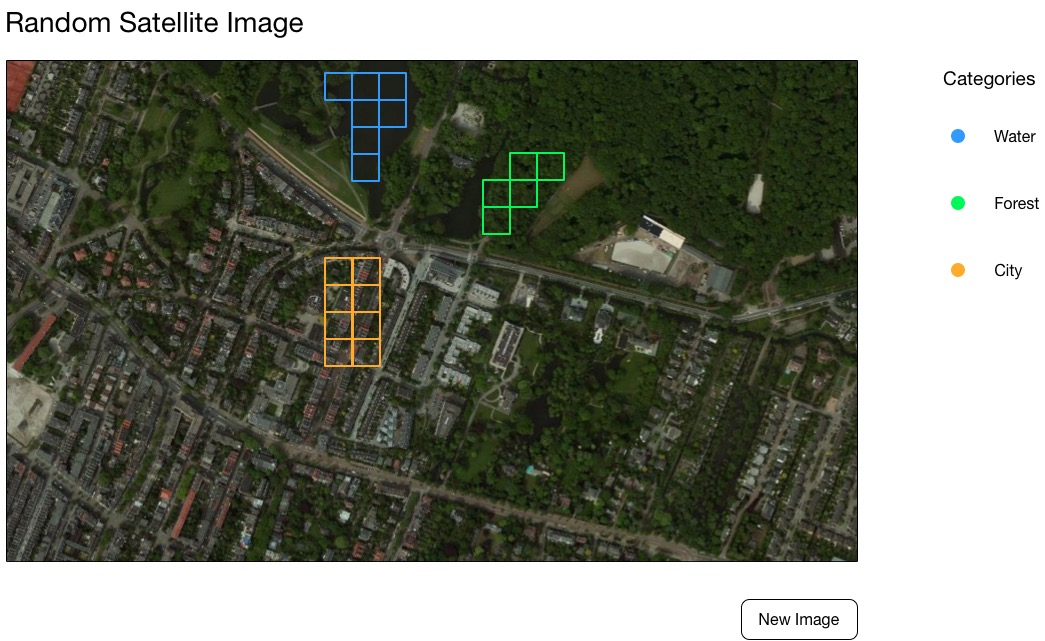
\includegraphics[width=0.8\textwidth]{impression.jpg}
    \caption{Impression of what the user interacts with and a possible outcome.}
	\label{fig:impression}
\end{figure}
\noindent
The most notable attention grabber is the satellite image. This image will be acquired through a random call from a homogenous satellite image database on every new instantiation of the system. Another possibility to acquire new data is by clicking on the 'New image' button.

Right of the satellite image one can see labels (Forest, City, Water) which correspond with the labels which are outputs of the classification. 

Results obtained from our algorithm, given the current satellite image as input, are graphically feed back to the user. The impression above does that by showing a correspondence between image patches and their respective label via color coding laid over the satellite image. This rendition just shows a few islands of resulsts as an example. Normally the entire image will have such arching (which will be a lot more subtle).\\
\\
Figure \ref{fig:grid} shows how it works internally. Two grids are maintained. One with patches the size of 25 by 25 pixels. The other by the size of 50 by 50 pixels. The latter is actually fed to the Neural Network from which will be decided for that patch the percentage of type of label it contains.  Four 50 by 50 pixels will be grouped together to create a square. In the middle the 25 by 25 pixels patch is placed. This patch will eventually be coloured on the satellite image to indicate the type of label. To decide that, a weighted majority vote of the four 50 by 50 pixels surrounding that smaller patch is computed. Like a convolution filter this construction is shifted over the satellite image as to decide for every area on it. As one can imagine, 25 pixels at the borders are omitted. 

\begin{figure}[h!]
    \centering
    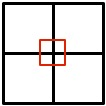
\includegraphics[scale=0.6]{grid.jpg}
    \caption{Grid structure which facilitates the algorithm.}
	\label{fig:grid}
\end{figure}

\section{MoSCoW}
Since a limited amount of time is available and we thought of quite some experiments and features that could be added, we used the MoSCoW method to get our priorities straight and focus on the most important requirements. MoSCow stands for \textit{Must have}, \textit{Should have}, \textit{Could have} and \textit{Would have}. All the requirements are labeled in these four classes.\\

\subsection{Must have}
Must have requirements are critical to project success. 
\begin{itemize}
\item Create code based on a \textit{Convolutional Neural Network} (CNN) that enables automatic classification of patches from satellite images. Considering images acquired on provincial level and a substantial amount of pixels in one patch (at least 50 x 50 pixels). 
\item At least the following classes should be recognized: vegetation, city and water. 
\item Develop a way to visualize the automatic classifications clearly.
\end{itemize}

\subsection{Should have}
Requirements labeled as should have are important to book success, but not necessary for delivery. 

\begin{itemize}
\item Create a clear interface in which the unlabeled images can be uploaded, and the output consists of labeled images. 
\item Calculate the uncertainty in the classification and ask user input for very uncertain patches.
\end{itemize}

\subsection{Could have}
It would be very nice if we would be able to reach the Could have feautures, but they are not critical. 
\begin{itemize}
\item Experiment with pre-processed images (noise reduction, gradient calculations)
\item Analyze images on city level, so with more details present. For this purpose new classes have to be added, such as roadways, cycle paths, 	buildings, distinct vegetations etc. 
\item Experiment with other models than the state-of-the art LeNet-1 CNN. For examples, a CNN in which Genetic Algorithms are incorporated, or implementing an Extreme Learning Machine for the training of the weights. 
\end{itemize}

\subsection{Would have}
These requirements are implemented only in the most ideal situation. They are considered as the dream project, sometimes serving as a suggestion for further projects. 

\begin{itemize}
\item Develop a method for high-detailed automatic vector graphics, in which segmentation of the distinct labeled classes is incorporated.
\item Use the input of the users to improve the automatic classification. 
\item Sell the software package to Google. 
\end{itemize}

\chapter{Implementation}

\section{Dataset}

\section{Convolutional Neural Network}
When we sat down and thought about the network architecture, we had to keep in mind the complexity of the network. Dealing with satellite imagery meant dealing with a large amount of data per image. In turn, this meant a large amount of connections between the input from the image data to the hidden layer, which leads to a large amount of parameters to tweak.
During our research phase, we encountered a variety of papers that touched on this subject. Most of these papers have one thing in common, which is their use of convolutional neural networks (CNN). Using convolution operations on small regions of the image, the previous problem could be avoided. Another advantage of using CNN is the ability to take into account correlations of neighboring input data, which are plentiful in satellite images. CNN also makes use of the principle of weight sharing in convolutional layers, which further reduces the amount of free parameters.

\subsection{LeNet-1}
One of the biggest advantages of using CNN, and especially LeCun's LeNet-1 implementation, is the incorporation of backpropagation learning. This meant that all the weights of the layers were adjusted iteratively, eliminating the need to manually create the convolution masks.

\chapter{Schedule}

\end{document}



